\documentclass[10pt,a4paper]{article}

% ---------------- Pacotes ----------------
\usepackage[utf8]{inputenc}
\usepackage[T1]{fontenc}
\usepackage[brazil]{babel}
\usepackage[a4paper,margin=2cm]{geometry}
\usepackage{graphicx}
\usepackage{booktabs}
\usepackage{tabularx}
\usepackage{array}
\usepackage{wrapfig}
\usepackage{float}
\usepackage{listings}
\usepackage{xcolor}
\usepackage{enumitem}
\usepackage{caption}
\usepackage[hidelinks]{hyperref}

% Espaçamento compacto (limite de 12 páginas)
\setlist{noitemsep,topsep=2pt}
\setlength{\parskip}{3pt}
\captionsetup{font=small,skip=4pt}
\setlength{\emergencystretch}{3em}

% Estilo do código SQL
\lstset{
  language=SQL,
  basicstyle=\ttfamily\scriptsize,
  keywordstyle=\color{blue!70!black}\bfseries,
  commentstyle=\color{gray},
  stringstyle=\color{red!60!black},
  morekeywords={STRAIGHT_JOIN,LIMIT,EXISTS,INDEX,DATETIME},
  frame=single,
  framesep=3pt,
  aboveskip=4pt,
  belowskip=4pt,
  breaklines=true,
  columns=fullflexible
}

\begin{document}

% ---------------- Cabeçalho (sem capa, como pede o enunciado) ----------------
\begin{center}
\textbf{UNIVERSIDADE FEDERAL DE MINAS GERAIS}\\
\textbf{INSTITUTO DE CIÊNCIAS EXATAS}\\
\textbf{DEPARTAMENTO DE CIÊNCIA DA COMPUTAÇÃO}\\
\textbf{DISCIPLINA: INTRODUÇÃO A BANCO DE DADOS}\\[6pt]
\textbf{TRABALHO PRÁTICO 2 -- Gestão de Médicos e Plantões}\\[6pt]
Grupo 5: Gustavo Abalem Tronconi Macedo, Isabelle de Matos Gonçalves,\\
Nicolle Salgado Silva e Paola Alves Ferreira
\end{center}

% =====================================================================
\section{Introdução}\label{sec:intro}
% ~0,6 página

Este trabalho apresenta o projeto e a implementação de um banco de dados relacional para a \textbf{gestão de profissionais de saúde e plantões} em uma rede de unidades hospitalares. Conforme o enunciado do Trabalho Prático~2 \cite{enunciado}, o banco foi projetado seguindo o processo visto em aula \cite{material,elmasri}: descrição do minimundo, projeto conceitual (diagrama ER), projeto lógico (esquema relacional com restrições de integridade), implementação no SGBD MySQL e comparação do desempenho de diferentes formulações SQL para dez consultas.

A Tabela~\ref{tab:requisitos} relaciona cada exigência do enunciado com a forma como foi atendida e a seção do relatório onde aparece.

\begin{table}[H]
\centering\footnotesize
\caption{Exigências do enunciado e como foram atendidas.}
\label{tab:requisitos}
\begin{tabularx}{\textwidth}{>{\raggedright\arraybackslash}p{5.6cm}Xc}
\toprule
Exigência do enunciado & Como foi atendida & Seção \\
\midrule
Diagrama ER com $\geq$ 4 entidades e $\geq$ 3 relacionamentos, sendo $\geq$ 1 M:N & 6 entidades e 6 relacionamentos, sendo 2 M:N (\emph{Escalado em} e \emph{Prescreve}) & \ref{sec:er} \\
Cada entidade com chave e $\geq$ 2 outros atributos & todas as entidades têm chave e de 2 a 5 atributos & \ref{sec:er} \\
$\geq$ 1 atributo multivalorado & \emph{especialidades} (Profissional) e \emph{contatos} (Paciente) & \ref{sec:er} \\
Relacionamento M:N com $\geq$ 1 atributo & \emph{funcao} em \emph{Escalado em}; \emph{dose} e \emph{frequencia} em \emph{Prescreve} & \ref{sec:er} \\
Esquema relacional com restrições de integridade & 10 tabelas com PK, FK (com ações referenciais), NOT NULL, UNIQUE, CHECK e 4 gatilhos & \ref{sec:logico} \\
Implementação no MySQL Workbench e no MySQL & MySQL 8 e MySQL Workbench & \ref{sec:implementacao} \\
Volume de dados suficiente para medir o desempenho & cerca de 3 milhões de linhas, das quais 1 milhão de atendimentos e 1,1 milhão de prescrições & \ref{sec:implementacao} \\
10 consultas: 2 de seleção/projeção, 3 com junção de 2 relações, 3 com junção de 3 ou mais, 2 com agregação sobre junção & Q1--Q2, Q3--Q5, Q6--Q8 e Q9--Q10, respectivamente & \ref{sec:consultas} \\
Cada consulta em $\geq$ 2 formas diferentes & 3 formas por consulta: índices, JOIN $\times$ subconsultas, ordem das relações e tabelas derivadas & \ref{sec:consultas} \\
Cada consulta executada $\geq$ 5 vezes, com tempo médio & 5 execuções por forma, com média, mediana e desvio padrão & \ref{sec:metodologia} \\
Especificação textual, SQL e desempenho de cada consulta & uma subseção por consulta, com tabela de tempos e análise do plano de execução & \ref{sec:consultas} \\
Autoavaliação com as tarefas de cada integrante & tabela de tarefas por integrante & \ref{sec:autoavaliacao} \\
\bottomrule
\end{tabularx}
\end{table}

O relatório está organizado da seguinte forma: a Seção~\ref{sec:minimundo} descreve o minimundo; as Seções~\ref{sec:er} e~\ref{sec:logico} apresentam os projetos conceitual e lógico; a Seção~\ref{sec:implementacao} trata da implementação e da carga de dados; as Seções~\ref{sec:metodologia} e~\ref{sec:consultas} descrevem a metodologia de medição e as dez consultas; a Seção~\ref{sec:conclusoes} reúne as conclusões; e a Seção~\ref{sec:autoavaliacao} traz a autoavaliação do grupo.

% =====================================================================
\section{Descrição do minimundo}\label{sec:minimundo}
% ~0,8 página

Uma rede de saúde deseja controlar seus profissionais, a escala de plantões das suas unidades e os atendimentos realizados aos pacientes, incluindo os remédios prescritos. A descrição a seguir é a base do diagrama ER da Figura~\ref{fig:er} \cite{elmasri}.

\textbf{Profissionais.} Cada profissional é identificado por um código e possui CPF (único), nome, cargo e carga horária semanal contratada. Os cargos possíveis são médico, enfermeiro, técnico de enfermagem e fisioterapeuta, e a carga horária fica entre 12 e 60 horas. Um profissional pode ter várias especialidades (por exemplo, Cardiologia e Pediatria) ou nenhuma.

\textbf{Unidades.} A rede é formada por unidades identificadas por um código, com nome (único) e tipo: hospital, UPA, policlínica ou maternidade.

\textbf{Plantões.} Cada plantão é identificado por um código e possui data, turno e duração. Os turnos são manhã (7h às 13h) e tarde (13h às 19h), com 6 horas, e noite (19h às 7h do dia seguinte), com 12 horas. Todo plantão ocorre em exatamente uma unidade, e cada unidade tem no máximo um plantão por dia e turno.

\textbf{Escala.} Um profissional pode ser escalado em vários plantões, e todo plantão tem pelo menos um profissional escalado. Para cada escala, registra-se a função exercida pelo profissional naquele plantão: coordenador, plantonista ou assistência.

\textbf{Pacientes.} Cada paciente é identificado por um código e possui CPF (único), nome, data de nascimento e um ou mais contatos (telefones ou e-mails).

\textbf{Atendimentos.} Cada atendimento é identificado por um código e possui data e hora, tipo (consulta, emergência, retorno ou procedimento) e diagnóstico. Todo atendimento é realizado por exatamente um profissional, prestado a exatamente um paciente e ocorre durante exatamente um plantão. Um mesmo profissional, paciente ou plantão pode estar associado a vários atendimentos.

\textbf{Remédios e prescrições.} Cada remédio é identificado por um código e possui nome, fabricante, princípio ativo e tarja (sem tarja, vermelha ou preta); não há dois remédios com o mesmo nome e fabricante. Em um atendimento podem ser prescritos vários remédios, e um remédio pode ser prescrito em vários atendimentos. Para cada prescrição, registram-se a dose e a frequência.

\textbf{Regras de negócio.} Além do que o diagrama ER representa, a aplicação deve respeitar as seguintes regras:
\begin{enumerate}[label=\textbf{R\arabic*.}]
  \item O profissional que realiza um atendimento deve estar escalado no plantão durante o qual o atendimento ocorre.
  \item A data e a hora do atendimento devem estar dentro do horário do plantão.
  \item Somente médicos podem prescrever remédios.
  \item Um plantão não pode ficar sem nenhum profissional escalado.
\end{enumerate}
Essas regras envolvem mais de uma tabela e não podem ser expressas no diagrama ER nem por restrições de chave. Por isso, foram implementadas com gatilhos \cite{mysql-trigger} (Seção~\ref{sec:restricoes}).

\textbf{Preservação do histórico.} Profissionais, pacientes, unidades e remédios que já aparecem em atendimentos ou plantões não podem ser excluídos. Já as especialidades, os contatos, as escalas e as prescrições são excluídos junto com o registro a que pertencem.
% =====================================================================
\section{Projeto conceitual (diagrama ER)}\label{sec:er}

O diagrama ER da Figura~\ref{fig:er}, em notação de Chen \cite{elmasri}, foi construído a partir do minimundo da Seção~\ref{sec:minimundo}. Ele tem 6 entidades (Profissional, Plantão, Unidade, Atendimento, Paciente e Remédio) e 6 relacionamentos. Dois deles são M:N com atributos próprios: \emph{Escalado em}, com a função do profissional no plantão, e \emph{Prescreve}, com a dose e a frequência. Os demais são 1:N: \emph{Ocorre em}, \emph{Realiza}, \emph{Recebe} e \emph{Ocorre durante}. Os atributos \emph{especialidades} e \emph{contatos} são multivalorados. As linhas duplas indicam participação total: todo atendimento tem um profissional, um paciente e um plantão, e todo plantão ocorre em uma unidade e tem ao menos um profissional escalado. O CPF de profissionais e pacientes é chave candidata, e os códigos foram escolhidos como identificadores.

\begin{figure}[H]
  \centering
  \includegraphics[width=0.9\textwidth]{ER_TP2_GRUPO_5.pdf}
  \caption{Diagrama ER do banco de dados (notação de Chen).}
  \label{fig:er}
\end{figure}

% =====================================================================
\section{Projeto lógico (esquema relacional)}\label{sec:logico}

O diagrama ER foi mapeado para o modelo relacional seguindo o algoritmo de mapeamento visto em aula \cite{elmasri,material}:
\begin{itemize}
  \item cada entidade virou uma tabela, com o seu identificador como chave primária;
  \item cada atributo multivalorado virou uma tabela própria, com chave composta pela chave da entidade e pelo valor;
  \item cada relacionamento 1:N virou uma chave estrangeira no lado N, \texttt{NOT NULL} quando a participação é total;
  \item cada relacionamento M:N virou uma tabela com as chaves das duas entidades, que juntas formam a chave primária, e com os atributos do relacionamento.
\end{itemize}
O esquema resultante tem 10 tabelas. As chaves primárias estão sublinhadas, e as chaves estrangeiras são indicadas com $\rightarrow$.

{\small
\begin{itemize}
  \item \textsc{Unidade}(\underline{id\_unidade}, nome, tipo)
  \item \textsc{Profissional}(\underline{id\_prof}, cpf, nome, cargo, carga\_horaria)
  \item \textsc{Profissional\_Especialidade}(\underline{id\_prof, especialidade}); id\_prof $\rightarrow$ Profissional
  \item \textsc{Plantao}(\underline{id\_plantao}, data, duracao\_h, turno, id\_unidade); id\_unidade $\rightarrow$ Unidade
  \item \textsc{Escalado\_Em}(\underline{id\_prof, id\_plantao}, funcao); id\_prof $\rightarrow$ Profissional; id\_plantao $\rightarrow$ Plantao
  \item \textsc{Paciente}(\underline{id\_paciente}, cpf, nome, data\_nasc)
  \item \textsc{Paciente\_Contato}(\underline{id\_paciente, contato}); id\_paciente $\rightarrow$ Paciente
  \item \textsc{Remedio}(\underline{id\_remedio}, nome, fabricante, principio\_ativo, tarja)
  \item \textsc{Atendimento}(\underline{id\_atend}, data\_hora, tipo, diagnostico, id\_prof, id\_paciente, id\_plantao); id\_prof $\rightarrow$ Profissional; id\_paciente $\rightarrow$ Paciente; id\_plantao $\rightarrow$ Plantao
  \item \textsc{Prescricao}(\underline{id\_atend, id\_remedio}, dose, frequencia); id\_atend $\rightarrow$ Atendimento; id\_remedio $\rightarrow$ Remedio
\end{itemize}}

\subsection{Restrições de integridade}\label{sec:restricoes}

A Tabela~\ref{tab:restricoes} resume as restrições declaradas no esquema. As restrições CHECK \cite{mysql-check} implementam os domínios descritos no minimundo.

\begin{table}[H]
\centering\footnotesize
\caption{Restrições de integridade do esquema.}
\label{tab:restricoes}
\begin{tabularx}{\textwidth}{lX}
\toprule
Tipo & Aplicação \\
\midrule
PRIMARY KEY & todas as tabelas; chave composta nas tabelas dos M:N e dos multivalorados \\
FOREIGN KEY & os 6 relacionamentos e os 2 multivalorados, com ações referenciais (Tabela~\ref{tab:fk}) \\
NOT NULL & atributos obrigatórios e chaves estrangeiras que representam participação total \\
UNIQUE & \texttt{cpf} (profissional e paciente); nome da unidade; (nome, fabricante) do remédio; (unidade, data, turno) do plantão \\
CHECK & cargo, turno, função, tipo de unidade, tipo de atendimento e tarja dentro dos valores do minimundo; CPF com 11 dígitos; carga horária entre 12 e 60 h; duração de 6 h (manhã/tarde) ou 12 h (noite) \\
Gatilhos & regras R1 a R4 da Seção~\ref{sec:minimundo} \\
\bottomrule
\end{tabularx}
\end{table}

As ações referenciais das chaves estrangeiras \cite{mysql-fk} estão na Tabela~\ref{tab:fk}. A \textbf{propagação} foi usada onde o registro dependente não tem sentido sozinho: as especialidades, os contatos, a escala de um plantão e as prescrições de um atendimento. O \textbf{bloqueio} preserva o histórico: não se exclui um profissional, paciente, unidade ou remédio que já aparece em atendimentos ou plantões. A \textbf{anulação} não foi usada, porque todas as chaves estrangeiras são \texttt{NOT NULL}: ou fazem parte da chave primária, ou representam participação total. Nas alterações, usou-se propagação em todas, para que uma eventual mudança de código se reflita nas tabelas que o referenciam.

\begin{table}[H]
\centering\footnotesize
\caption{Ações referenciais das chaves estrangeiras.}
\label{tab:fk}
\begin{tabular}{llcc}
\toprule
Chave estrangeira & Referencia & Exclusão & Alteração \\
\midrule
profissional\_especialidade.id\_prof & profissional & propagação & propagação \\
paciente\_contato.id\_paciente & paciente & propagação & propagação \\
plantao.id\_unidade & unidade & bloqueio & propagação \\
escalado\_em.id\_prof & profissional & bloqueio & propagação \\
escalado\_em.id\_plantao & plantao & propagação & propagação \\
atendimento.id\_prof & profissional & bloqueio & propagação \\
atendimento.id\_paciente & paciente & bloqueio & propagação \\
atendimento.id\_plantao & plantao & bloqueio & propagação \\
prescricao.id\_atend & atendimento & propagação & propagação \\
prescricao.id\_remedio & remedio & bloqueio & propagação \\
\bottomrule
\end{tabular}
\end{table}

As regras R1 a R4 foram implementadas com gatilhos \cite{mysql-trigger}. Cada regra pode ser violada por operações em mais de uma tabela, e por isso é verificada em todas elas. R1 (profissional escalado no plantão) é verificada nas inclusões e alterações de \texttt{atendimento} e nas exclusões e alterações de \texttt{escalado\_em}: não se pode tirar da escala quem já atendeu naquele plantão. R2 (horário do plantão) é verificada nas inclusões e alterações de \texttt{atendimento} e nas alterações de data, turno ou duração de \texttt{plantao}. R3 (só médicos prescrevem) é verificada em \texttt{prescricao}, na troca do profissional de um atendimento com prescrição e na mudança de cargo de um médico que já prescreveu. R4 (plantão com ao menos um escalado) é verificada nas exclusões e alterações de \texttt{escalado\_em}. Uma operação que viole uma regra é recusada com o erro 1644 e uma mensagem que identifica a regra, como ``R3: somente médicos podem prescrever remédios''. A única situação que o MySQL não consegue impedir é a \emph{criação} de um plantão sem ninguém escalado, porque isso exigiria verificar a regra no fim da transação, recurso que o MySQL não oferece. Para esse caso, foi criado o procedimento \texttt{criar\_plantao}, que insere o plantão e o seu coordenador numa única transação e é a forma prevista de criar plantões.

% =====================================================================
\section{Implementação e carga de dados}\label{sec:implementacao}

O banco foi criado no MySQL~8 com o MySQL Workbench, conforme o enunciado \cite{enunciado}. Os scripts são: \texttt{01\_esquema.sql} (tabelas e restrições), \texttt{02\_carregar\_dados.sql} (carga com \texttt{LOAD DATA}), \texttt{03\_consultas.sql} (as 30 formas das consultas) e \texttt{04\_gatilhos.sql} (regras de negócio). \textbf{Ambiente:} % processador, memória, sistema operacional, versão do MySQL

\begin{wraptable}{r}{0.36\textwidth}
\vspace{-10pt}\centering\footnotesize
\caption{Volume de dados carregado.}
\label{tab:volume}
\begin{tabular}{lr}
\toprule
Tabela & Linhas \\
\midrule
unidade & 40 \\
profissional & 10.000 \\
profissional\_especialidade & 8.451 \\
plantao & 83.334 \\
escalado\_em & 249.812 \\
paciente & 200.000 \\
paciente\_contato & 310.191 \\
remedio & 154 \\
atendimento & 1.000.000 \\
prescricao & 1.104.897 \\
\midrule
\textbf{Total} & \textbf{2.966.879} \\
\bottomrule
\end{tabular}
\vspace{-8pt}
\end{wraptable}

Os dados foram gerados por um script próprio em Python (\texttt{gerar\_dados.py}), opção permitida pelo enunciado, que admite dados reais ou gerados sinteticamente \cite{enunciado}. Optou-se por não usar bases públicas porque as bases de saúde disponíveis não têm a estrutura do minimundo (escalas de plantão ligadas a unidades, atendimentos e prescrições) e omitem dados pessoais como nome e CPF, que são protegidos pela LGPD \cite{lgpd}. Também não se usou um gerador genérico, como o Spawner, porque ele preenche cada tabela de forma independente e não garantiria as regras R1 a R4. O script gera dados coerentes com todas as restrições e regras do modelo: os profissionais atendem apenas nos plantões em que estão escalados e dentro do horário do turno, só médicos prescrevem e pediatras atendem crianças. Como a semente é fixa, os mesmos dados são produzidos a cada execução, o que permite repetir as medições. O volume carregado está na Tabela~\ref{tab:volume}.



% =====================================================================
% Substitui, no main.tex, as seções "Metodologia de medição",
% "Consultas e análise de desempenho" e "Análise geral e conclusões".
% Números: tempos.csv (5 execuções por forma). Os planos citados vêm
% do explain.txt.
% =====================================================================

\section{Metodologia de medição}\label{sec:metodologia}

As medições foram feitas por um script em Python (\texttt{medir\_tempos.py}, conector \texttt{mysql-connector-python}). Cada forma de cada consulta foi executada 5 vezes seguidas, e o relatório traz a média, como pede o enunciado, junto com a mediana, o desvio padrão e o tempo da 1ª execução. Esse último valor mostra o efeito de \emph{cold start}: na primeira vez, as páginas de dados e de índice ainda não estão na memória. Quando a 1ª execução destoa muito das demais, a mediana representa melhor o tempo típico, e as análises usam a mediana nesses casos. O tempo medido inclui a execução no servidor e a transferência de todas as linhas para o cliente.

Os índices usados por uma forma foram criados imediatamente antes dela e removidos logo depois, para não interferir nas demais. O plano de execução de cada forma foi obtido com \texttt{EXPLAIN} \cite{mysql-explain}. O script também comparou o conteúdo completo dos resultados: as três formas de cada consulta devolveram exatamente as mesmas linhas. Os índices que o InnoDB cria automaticamente para as chaves primárias e estrangeiras \cite{mysql-fk} existem em todas as formas.

\textbf{Ambiente:} % processador, memória, Ubuntu 24.04 (?), MySQL 8.x (versão exata: SELECT VERSION();)

As Tabelas~\ref{tab:q1} a~\ref{tab:q10} trazem os tempos de cada consulta. A coluna \textbf{vs.\ (a)} dessas tabelas é a razão entre a média da forma e a média da forma (a): 0,25x significa 4 vezes mais rápida, e 2,00x significa 2 vezes mais lenta.

% =====================================================================
\section{Consultas e análise de desempenho}\label{sec:consultas}

% ------------------------------------------------------------------
\subsection{Q1 -- Seleção e projeção}
\textbf{Especificação:} nome e CPF dos médicos com carga horária de pelo menos 36 horas.

\begin{lstlisting}
-- Q1a: sem indice auxiliar
SELECT nome, cpf FROM profissional WHERE cargo = 'Medico' AND carga_horaria >= 36;
-- Q1b: mesma consulta apos
CREATE INDEX idx_prof_cargo_carga ON profissional (cargo, carga_horaria);
-- Q1c: mesma consulta apos (indice de cobertura)
CREATE INDEX idx_prof_cobertura ON profissional (cargo, carga_horaria, nome, cpf);
\end{lstlisting}

\begin{table}[H]\centering\footnotesize
\caption{Tempos das formas da Q1 (ms, 5 execuções).}\label{tab:q1}
\begin{tabular}{llrrrrr}\toprule
Forma & Descrição & Média & Mediana & Desvio & 1ª exec. & vs.\ (a) \\ \midrule
Q1a & sem índice           & 29,2 & 28,7 & 1,2 & 31,2 & 1,00x \\
Q1b & índice composto      & 29,4 & 29,0 & 0,9 & 31,0 & 1,01x \\
Q1c & índice de cobertura  & 29,7 & 28,1 & 3,7 & 36,3 & 1,02x \\ \bottomrule
\end{tabular}
\end{table}

\textbf{Resultado:} 2.250 linhas. Exemplo: (Alice Almeida Lima, 46786138705); (Alice Andrade Faria, 35483421329); (Alice Batista Lopes, 26438185124).

\textbf{Análise (Tabela~\ref{tab:q1}):} os planos mudaram como esperado. Sem índice, a tabela inteira é lida (\texttt{ALL}, 10.094 linhas). Com o índice composto, há uma busca por intervalo (\texttt{range}). Com o índice de cobertura, o \texttt{EXPLAIN} mostra \emph{Using index}: a consulta é respondida só pelo índice, sem ler a tabela. Ainda assim, os tempos são praticamente iguais. A tabela é pequena (10 mil linhas) e fica inteira na memória, e o filtro seleciona 22\% das linhas. Assim, o tempo é dominado pela transferência das 2.250 linhas do resultado, e não pela busca. Conclusão: o índice só traz ganho perceptível em tabelas grandes ou com filtros seletivos.

% ------------------------------------------------------------------
\subsection{Q2 -- Seleção e projeção}
\textbf{Especificação:} código, data, duração e unidade dos plantões noturnos de março de 2025.

\begin{lstlisting}
-- Q2a: sem indice auxiliar
SELECT id_plantao, data, duracao_h, id_unidade FROM plantao
WHERE turno = 'Noite' AND data BETWEEN DATE '2025-03-01' AND DATE '2025-03-31';
-- Q2b: mesma consulta apos
CREATE INDEX idx_plantao_turno_data ON plantao (turno, data);
-- Q2c: com o mesmo indice, filtrando a data com funcoes
... WHERE turno = 'Noite' AND YEAR(data) = 2025 AND MONTH(data) = 3;
\end{lstlisting}

\begin{table}[H]\centering\footnotesize
\caption{Tempos das formas da Q2 (ms, 5 execuções).}\label{tab:q2}
\begin{tabular}{llrrrrr}\toprule
Forma & Descrição & Média & Mediana & Desvio & 1ª exec. & vs.\ (a) \\ \midrule
Q2a & BETWEEN sem índice         & 78,2 & 75,9 & 9,8 & 75,9 & 1,00x \\
Q2b & BETWEEN com índice         & 18,9 & 18,5 & 1,3 & 21,1 & 0,24x \\
Q2c & YEAR()/MONTH() com índice  & 32,8 & 32,7 & 0,1 & 32,7 & 0,42x \\ \bottomrule
\end{tabular}
\end{table}

\textbf{Resultado:} 1.054 linhas. Exemplo: (48453, 2025-03-01, 12, 1); (48458, 2025-03-01, 12, 3); (48461, 2025-03-01, 12, 4).

\textbf{Análise (Tabela~\ref{tab:q2}):} sem índice, as 83 mil linhas de \texttt{plantao} são lidas. Com o índice (turno, data), o MySQL percorre só o intervalo desejado (1.054 linhas), e a consulta fica 4 vezes mais rápida. Na forma (c), as funções \texttt{YEAR()} e \texttt{MONTH()} aplicadas à coluna impedem a busca por intervalo de datas: o índice é usado apenas para o turno (\texttt{ref}, cerca de 41,7 mil linhas estimadas), e o restante é filtrado linha a linha. Ela é 1,7 vez mais lenta que a (b), embora ainda mais rápida que a (a), porque restringe ao turno da noite. O resultado mostra que um filtro com função sobre a coluna anula boa parte do benefício do índice.

% ------------------------------------------------------------------
\subsection{Q3 -- Junção de duas relações}
\textbf{Especificação:} plantões ocorridos em unidades do tipo UPA, com o nome da unidade.

\begin{lstlisting}
-- Q3a: JOIN explicito
SELECT p.id_plantao, p.data, p.turno, u.nome AS unidade
FROM plantao p JOIN unidade u ON u.id_unidade = p.id_unidade WHERE u.tipo = 'UPA';
-- Q3b: juncao no WHERE, ordem invertida no FROM
... FROM unidade u, plantao p WHERE u.id_unidade = p.id_unidade AND u.tipo = 'UPA';
-- Q3c: subconsulta IN + subconsulta escalar para o nome
SELECT p.id_plantao, p.data, p.turno,
       (SELECT u.nome FROM unidade u WHERE u.id_unidade = p.id_unidade) AS unidade
FROM plantao p WHERE p.id_unidade IN (SELECT id_unidade FROM unidade WHERE tipo = 'UPA');
\end{lstlisting}

\begin{table}[H]\centering\footnotesize
\caption{Tempos das formas da Q3 (ms, 5 execuções).}\label{tab:q3}
\begin{tabular}{llrrrrr}\toprule
Forma & Descrição & Média & Mediana & Desvio & 1ª exec. & vs.\ (a) \\ \midrule
Q3a & JOIN explícito              & 769,0 & 740,2 & 60,0 & 865,4 & 1,00x \\
Q3b & WHERE, FROM invertido       & 718,9 & 714,4 &  9,2 & 719,4 & 0,93x \\
Q3c & subconsultas IN e escalar   & 726,4 & 721,5 & 13,6 & 709,8 & 0,94x \\ \bottomrule
\end{tabular}
\end{table}

\textbf{Resultado:} 46.053 linhas. Exemplo: (6, 2024-01-01, Manha, UPA Leste 01); (7, 2024-01-01, Tarde, UPA Leste 01); (8, 2024-01-01, Noite, UPA Leste 01).

\textbf{Análise (Tabela~\ref{tab:q3}):} as formas (a) e (b) têm planos idênticos. O otimizador reordena as junções sozinho: começa por \texttt{unidade} (40 linhas, filtradas por tipo) e acessa \texttt{plantao} pelo índice de \texttt{(id\_unidade, data, turno)}, independentemente da ordem escrita no \texttt{FROM}. Na forma (c), o \texttt{IN} é transformado em semijunção com o mesmo plano, e a subconsulta escalar faz uma busca pela chave primária por linha, de custo pequeno. A diferença de 6--7\% nas médias vem da 1ª execução da forma (a) (\emph{cold start}); as medianas são próximas. Com 46 mil linhas no resultado, a transferência domina o tempo.

% ------------------------------------------------------------------
\subsection{Q4 -- Junção de duas relações}
\textbf{Especificação:} atendimento, remédio, dose e frequência das prescrições de remédios de tarja preta.

\begin{lstlisting}
-- Q4a: JOIN (ordem escolhida pelo otimizador)
SELECT pr.id_atend, r.nome AS remedio, pr.dose, pr.frequencia
FROM prescricao pr JOIN remedio r ON r.id_remedio = pr.id_remedio WHERE r.tarja = 'Preta';
-- Q4b: STRAIGHT_JOIN forca comecar por prescricao
... FROM prescricao pr STRAIGHT_JOIN remedio r ON r.id_remedio = pr.id_remedio ...
-- Q4c: tabela derivada filtra os remedios antes da juncao
... FROM (SELECT id_remedio, nome FROM remedio WHERE tarja = 'Preta') r
    JOIN prescricao pr ON pr.id_remedio = r.id_remedio;
\end{lstlisting}

\begin{table}[H]\centering\footnotesize
\caption{Tempos das formas da Q4 (ms, 5 execuções).}\label{tab:q4}
\begin{tabular}{llrrrrr}\toprule
Forma & Descrição & Média & Mediana & Desvio & 1ª exec. & vs.\ (a) \\ \midrule
Q4a & JOIN                     & 3217,2 & 2948,0 & 655,4 & 4387,4 & 1,00x \\
Q4b & STRAIGHT\_JOIN           & 3760,6 & 3771,9 & 122,7 & 3583,8 & 1,17x \\
Q4c & tabela derivada filtrada & 2992,0 & 2949,4 &  87,2 & 2949,4 & 0,93x \\ \bottomrule
\end{tabular}
\end{table}

\textbf{Resultado:} 193.787 linhas. Exemplo: (2, Zolpidem 5 mg, 5 mg, 1x ao dia); (21, Morfina 5 mg, 2 comprimidos, 4/4h); (27, Midazolam 5 mg, 1 comprimido, 1x ao dia).

\textbf{Análise (Tabela~\ref{tab:q4}):} as formas (a) e (c) têm o mesmo plano, porque o MySQL incorpora a tabela derivada à consulta principal \cite{mysql-derived}: o plano começa por \texttt{remedio} (154 linhas, filtradas pela tarja) e busca as prescrições pelo índice da chave estrangeira. As medianas são praticamente iguais (2.948 e 2.949 ms). A média de (a) é maior apenas por causa da 1ª execução (\emph{cold start}). Na forma (b), o \texttt{STRAIGHT\_JOIN} obriga a ler as 1,1 milhão de prescrições e buscar o remédio de cada uma. Ela fica 28\% mais lenta pela mediana, porque o MySQL não pode mais escolher a ordem mais eficiente.

% ------------------------------------------------------------------
\subsection{Q5 -- Junção de duas relações}
\textbf{Especificação:} nome e CPF dos pacientes nascidos antes de 1950 e data/hora dos seus atendimentos de retorno com diagnóstico de diabetes.

\begin{lstlisting}
-- Q5a: JOIN sem indice auxiliar
SELECT pa.nome, pa.cpf, a.data_hora
FROM atendimento a JOIN paciente pa ON pa.id_paciente = a.id_paciente
WHERE a.tipo = 'Retorno' AND a.diagnostico = 'Diabetes'
  AND pa.data_nasc < DATE '1950-01-01';
-- Q5b: mesma consulta apos
CREATE INDEX idx_atend_tipo_diag ON atendimento (tipo, diagnostico);
-- Q5c: STRAIGHT_JOIN forca comecar por paciente
... FROM paciente pa STRAIGHT_JOIN atendimento a ON a.id_paciente = pa.id_paciente ...
\end{lstlisting}

\begin{table}[H]\centering\footnotesize
\caption{Tempos das formas da Q5 (ms, 5 execuções).}\label{tab:q5}
\begin{tabular}{llrrrrr}\toprule
Forma & Descrição & Média & Mediana & Desvio & 1ª exec. & vs.\ (a) \\ \midrule
Q5a & JOIN sem índice              &  915,6 &  904,9 &  34,6 &  957,9 & 1,00x \\
Q5b & índice (tipo, diagnostico)   &  300,6 &  123,0 & 432,1 & 1072,5 & 0,33x \\
Q5c & STRAIGHT\_JOIN por paciente  & 1750,8 & 1349,6 & 967,4 & 3480,3 & 1,91x \\ \bottomrule
\end{tabular}
\end{table}

\textbf{Resultado:} 1.285 linhas. Exemplo: (Ricardo Correia Machado, 48349436743, 2024-01-01 17:33); (Vanessa Fonseca Martins, 22892902622, 2024-01-02 11:26); (Natalia Duarte Batista, 49658529402, 2024-01-02 13:16).

\textbf{Análise (Tabela~\ref{tab:q5}):} sem índice, o MySQL lê o 1 milhão de atendimentos para encontrar 1\% deles. Com o índice (tipo, diagnostico), ele vai direto às cerca de 10,9 mil linhas candidatas. Pela mediana, a consulta fica 7,4 vezes mais rápida (123 ms contra 905 ms). A 1ª execução da forma (b) foi lenta (1.072 ms) porque o índice tinha acabado de ser criado e suas páginas ainda não estavam na memória. É um caso claro de \emph{cold start}, e é por isso que a mediana representa melhor essa forma. Na forma (c), começar por \texttt{paciente} obriga a ler os 200 mil pacientes e buscar os atendimentos de cada um nascido antes de 1950. Ela fica cerca de 1,5 vez mais lenta que a forma (a) pela mediana.

% ------------------------------------------------------------------
\subsection{Q6 -- Junção de cinco relações}
\textbf{Especificação:} atendimentos de emergência com diagnóstico de fratura, com paciente, profissional, unidade e data/hora.

\begin{lstlisting}
-- Q6a: JOINs encadeados
SELECT a.id_atend, a.data_hora, pa.nome AS paciente, pf.nome AS profissional,
       u.nome AS unidade
FROM atendimento a
JOIN paciente pa     ON pa.id_paciente = a.id_paciente
JOIN profissional pf ON pf.id_prof = a.id_prof
JOIN plantao pl      ON pl.id_plantao = a.id_plantao
JOIN unidade u       ON u.id_unidade = pl.id_unidade
WHERE a.tipo = 'Emergencia' AND a.diagnostico = 'Fratura';
-- Q6b: subconsultas escalares correlacionadas no SELECT
SELECT a.id_atend, a.data_hora,
  (SELECT nome FROM paciente WHERE id_paciente = a.id_paciente) AS paciente, ...
-- Q6c: forma (a) apos
CREATE INDEX idx_atend_tipo_diag ON atendimento (tipo, diagnostico);
\end{lstlisting}

\begin{table}[H]\centering\footnotesize
\caption{Tempos das formas da Q6 (ms, 5 execuções).}\label{tab:q6}
\begin{tabular}{llrrrrr}\toprule
Forma & Descrição & Média & Mediana & Desvio & 1ª exec. & vs.\ (a) \\ \midrule
Q6a & JOINs encadeados           & 1241,2 & 1216,2 &  39,0 & 1302,6 & 1,00x \\
Q6b & subconsultas escalares     & 1282,2 & 1258,4 &  42,2 & 1255,7 & 1,03x \\
Q6c & JOINs + índice             &  582,7 &  483,1 & 276,8 & 1072,4 & 0,47x \\ \bottomrule
\end{tabular}
\end{table}

\textbf{Resultado:} 17.890 linhas. Exemplo: (125, 2024-01-01 16:27, Marcos Castro Ferreira, Sara Rocha Lima, UPA Oeste 01); (185, 2024-01-01 08:28, Henrique Moura Fonseca, Tiago Duarte Costa, UPA Barreiro 01).

\textbf{Análise (Tabela~\ref{tab:q6}):} nas formas (a) e (b), o custo principal é a leitura completa de \texttt{atendimento}. As quatro junções restantes são buscas pela chave primária (\texttt{eq\_ref}), e é exatamente o mesmo trabalho que as subconsultas escalares da forma (b) fazem. Por isso as duas têm desempenho equivalente. O índice (tipo, diagnostico) da forma (c) substitui a leitura de 1 milhão de linhas pela leitura de cerca de 35 mil, e a consulta fica 2,5 vezes mais rápida pela mediana. A 1ª execução, de novo mais lenta, mostra o \emph{cold start} do índice recém-criado.

% ------------------------------------------------------------------
\subsection{Q7 -- Junção de três relações}
\textbf{Especificação:} pacientes (nome e data de nascimento) atendidos em 2025 por profissionais com especialidade em Pediatria.

\begin{lstlisting}
-- Q7a: JOIN + DISTINCT
SELECT DISTINCT p.id_paciente, p.nome, p.data_nasc
FROM paciente p
JOIN atendimento a ON a.id_paciente = p.id_paciente
JOIN profissional_especialidade e ON e.id_prof = a.id_prof
WHERE e.especialidade = 'Pediatria'
  AND a.data_hora >= TIMESTAMP '2025-01-01 00:00:00'
  AND a.data_hora <  TIMESTAMP '2026-01-01 00:00:00';
-- Q7b: WHERE EXISTS (SELECT 1 FROM atendimento a JOIN profissional_especialidade e ...
--                    WHERE a.id_paciente = p.id_paciente AND ...)
-- Q7c: WHERE p.id_paciente IN (SELECT a.id_paciente FROM atendimento a JOIN ...)
\end{lstlisting}

\begin{table}[H]\centering\footnotesize
\caption{Tempos das formas da Q7 (ms, 5 execuções).}\label{tab:q7}
\begin{tabular}{llrrrrr}\toprule
Forma & Descrição & Média & Mediana & Desvio & 1ª exec. & vs.\ (a) \\ \midrule
Q7a & JOIN + DISTINCT  & 992,1 & 946,2 & 98,3 & 1162,4 & 1,00x \\
Q7b & EXISTS           & 758,1 & 741,5 & 27,7 &  737,2 & 0,76x \\
Q7c & IN               & 781,0 & 766,6 & 33,2 &  763,4 & 0,79x \\ \bottomrule
\end{tabular}
\end{table}

\textbf{Resultado:} 22.388 linhas. Exemplo: (22, Amanda Dias Nunes, 2012-06-19); (55, Laura Ribeiro Andrade, 2013-12-28); (77, Henrique Santos Cardoso, 2014-08-07). Os pacientes de pediatras são crianças, como prevê o minimundo.

\textbf{Análise (Tabela~\ref{tab:q7}):} na forma (a), a junção gera uma linha para cada atendimento, e o \texttt{DISTINCT} precisa de uma tabela temporária para eliminar os pacientes repetidos (\emph{Using temporary}). Nas formas (b) e (c), o MySQL~8 converte tanto o \texttt{EXISTS} quanto o \texttt{IN} em semijunção com materialização \cite{mysql-semijoin}. Os dois planos são idênticos: o conjunto de pacientes é calculado uma vez, sem duplicatas, e depois juntado a \texttt{paciente}. Isso explica o ganho de cerca de 24\% das formas (b) e (c), e também por que elas têm o mesmo desempenho entre si.

% ------------------------------------------------------------------
\subsection{Q8 -- Junção de quatro relações}
\textbf{Especificação:} profissionais que atuaram como coordenadores em plantões noturnos de UPAs em 2025, com a data do plantão e o nome da unidade.

\begin{lstlisting}
-- Q8a: JOINs sem indice auxiliar
SELECT pf.nome AS profissional, pf.cpf, pl.data, u.nome AS unidade
FROM profissional pf
JOIN escalado_em e ON e.id_prof = pf.id_prof
JOIN plantao pl    ON pl.id_plantao = e.id_plantao
JOIN unidade u     ON u.id_unidade = pl.id_unidade
WHERE e.funcao = 'Coordenador' AND pl.turno = 'Noite' AND u.tipo = 'UPA'
  AND pl.data BETWEEN DATE '2025-01-01' AND DATE '2025-12-31';
-- Q8b: forma (a) apos
CREATE INDEX idx_plantao_turno_data ON plantao (turno, data);
-- Q8c: ordem forcada unidade -> plantao -> escalado_em -> profissional
... FROM unidade u STRAIGHT_JOIN plantao pl ON ... STRAIGHT_JOIN escalado_em e ON ...
\end{lstlisting}

\begin{table}[H]\centering\footnotesize
\caption{Tempos das formas da Q8 (ms, 5 execuções).}\label{tab:q8}
\begin{tabular}{llrrrrr}\toprule
Forma & Descrição & Média & Mediana & Desvio & 1ª exec. & vs.\ (a) \\ \midrule
Q8a & JOINs sem índice    & 277,0 & 201,5 & 144,3 & 526,8 & 1,00x \\
Q8b & índice (turno, data)& 190,7 & 190,0 &   3,6 & 196,6 & 0,69x \\
Q8c & STRAIGHT\_JOIN      & 188,8 & 188,9 &   1,2 & 189,5 & 0,68x \\ \bottomrule
\end{tabular}
\end{table}

\textbf{Resultado:} 7.665 linhas (um coordenador por plantão noturno de UPA em 2025). Exemplo: (Daniel Barbosa Monteiro, 77664348900, 2025-01-01, UPA Barreiro 01); (Eduarda Oliveira Moreira, 92455836274, 2025-01-01, UPA Barreiro 02).

\textbf{Análise (Tabela~\ref{tab:q8}):} os três planos são iguais. O otimizador já começa por \texttt{unidade} (filtro de UPAs) e segue para \texttt{plantao} pelo índice que começa por \texttt{id\_unidade}. O índice (turno, data) aparece entre os possíveis (\emph{possible\_keys}), mas não foi escolhido. O \texttt{STRAIGHT\_JOIN} forçou exatamente a ordem que o otimizador já usava. A diferença nas médias vem só da 1ª execução da forma (a) (527 ms, \emph{cold start}); as medianas são iguais (cerca de 190 ms). É um resultado válido: criar um índice não garante que ele será usado, e forçar a ordem só ajuda quando o otimizador erra.

% ------------------------------------------------------------------
\subsection{Q9 -- Agregação sobre junção de três relações}
\textbf{Especificação:} quantidade de atendimentos por unidade, apenas unidades com mais de 30.000 atendimentos, da maior para a menor.

\begin{lstlisting}
-- Q9a: junta tudo e depois agrupa
SELECT u.id_unidade, u.nome, COUNT(*) AS total_atendimentos
FROM atendimento a JOIN plantao p ON p.id_plantao = a.id_plantao
JOIN unidade u ON u.id_unidade = p.id_unidade
GROUP BY u.id_unidade, u.nome HAVING COUNT(*) > 30000
ORDER BY total_atendimentos DESC;
-- Q9b: agrega primeiro (tabela derivada) e depois junta com unidade
SELECT u.id_unidade, u.nome, t.total_atendimentos FROM unidade u
JOIN (SELECT p.id_unidade, COUNT(*) AS total_atendimentos
        FROM atendimento a JOIN plantao p ON p.id_plantao = a.id_plantao
       GROUP BY p.id_unidade HAVING COUNT(*) > 30000) t ON t.id_unidade = u.id_unidade
ORDER BY t.total_atendimentos DESC;
-- Q9c: subconsulta correlacionada conta os atendimentos de cada unidade
\end{lstlisting}

\begin{table}[H]\centering\footnotesize
\caption{Tempos das formas da Q9 (ms, 5 execuções).}\label{tab:q9}
\begin{tabular}{llrrrrr}\toprule
Forma & Descrição & Média & Mediana & Desvio & 1ª exec. & vs.\ (a) \\ \midrule
Q9a & junta e agrupa              & 6518,3 & 6477,8 & 101,4 & 6699,4 & 1,00x \\
Q9b & agrega antes de juntar      &  763,6 &  764,3 &   1,7 &  764,4 & 0,12x \\
Q9c & subconsulta correlacionada  &  674,0 &  673,9 &   0,7 &  674,1 & 0,10x \\ \bottomrule
\end{tabular}
\end{table}

\textbf{Resultado:} 11 linhas. As cinco primeiras: (10, UPA Noroeste 01, 59.295); (32, UPA Sul 04, 55.137); (4, UPA Oeste 01, 47.922); (29, UPA Nordeste 03, 36.966); (40, UPA Noroeste 04, 36.376).

\textbf{Análise (Tabela~\ref{tab:q9}):} foi a maior diferença do trabalho. Na forma (a), o 1 milhão de linhas da junção é agrupado numa tabela temporária, com chave (id\_unidade, nome), sendo o nome um texto de até 100 caracteres (\emph{Using temporary; Using filesort}). Na forma (b), a contagem é feita antes da junção com \texttt{unidade}, agrupando só pelo inteiro \texttt{id\_unidade}. Como o índice de \texttt{plantao} começa por esse campo, as linhas já chegam agrupadas, e só 40 grupos são juntados depois. A consulta fica 8,5 vezes mais rápida. Na forma (c), cada uma das 40 unidades faz uma contagem usando apenas índices (\emph{Using index}), sem tabela temporária, e é 9,7 vezes mais rápida que a (a). Lição: agregar antes de juntar, e agrupar por uma chave estreita, reduz drasticamente o custo.

% ------------------------------------------------------------------
\subsection{Q10 -- Agregação sobre junção de três relações}
\textbf{Especificação:} os 10 remédios mais prescritos em atendimentos de emergência, com o princípio ativo e o número de prescrições.

\begin{lstlisting}
-- Q10a: JOIN das tres relacoes
SELECT r.id_remedio, r.nome, r.principio_ativo, COUNT(*) AS total_prescricoes
FROM prescricao pr JOIN atendimento a ON a.id_atend = pr.id_atend
JOIN remedio r ON r.id_remedio = pr.id_remedio
WHERE a.tipo = 'Emergencia'
GROUP BY r.id_remedio, r.nome, r.principio_ativo
ORDER BY total_prescricoes DESC, r.id_remedio LIMIT 10;
-- Q10b: ... WHERE pr.id_atend IN (SELECT id_atend FROM atendimento
--                                WHERE tipo = 'Emergencia') ...
-- Q10c: forma (a) apos
CREATE INDEX idx_atend_tipo ON atendimento (tipo);
\end{lstlisting}

\begin{table}[H]\centering\footnotesize
\caption{Tempos das formas da Q10 (ms, 5 execuções).}\label{tab:q10}
\begin{tabular}{llrrrrr}\toprule
Forma & Descrição & Média & Mediana & Desvio & 1ª exec. & vs.\ (a) \\ \midrule
Q10a & JOIN             & 5062,6 & 4966,2 & 211,2 &  5440,3 & 1,00x \\
Q10b & subconsulta IN   & 4989,0 & 4984,3 &  14,3 &  5004,6 & 0,99x \\
Q10c & JOIN + índice    & 8966,7 & 8644,3 & 709,2 & 10229,3 & 1,77x \\ \bottomrule
\end{tabular}
\end{table}

\textbf{Resultado:} 10 linhas. As três primeiras: (144, Sulfato ferroso 250 mg, Sulfato ferroso, 3.431); (36, Azitromicina 1 g, Azitromicina, 3.361); (61, Enalapril 1 g, Enalapril, 3.356).

\textbf{Análise (Tabela~\ref{tab:q10}):} as formas (a) e (b) têm planos idênticos: o \texttt{IN} vira uma semijunção, que, por ser feita sobre a chave primária, equivale à junção. As duas leem o 1 milhão de atendimentos, filtram as emergências e agrupam. Na forma (c), o índice em \texttt{tipo} \textbf{piorou} a consulta em 77\%. A coluna tem só 4 valores, e o índice levou o otimizador a mudar de plano: ele passou a começar por \texttt{remedio}, a ler as 1,1 milhão de prescrições pelo índice da chave estrangeira e a buscar o atendimento de cada uma para conferir o tipo. São mais de um milhão de acessos aleatórios à tabela \texttt{atendimento}, contra uma leitura sequencial na forma (a). O caso mostra que índice em coluna pouco seletiva pode atrapalhar, porque induz o otimizador a um plano pior \cite{elmasri,mysql-indexes}.

% =====================================================================
\section{Análise geral e conclusões}\label{sec:conclusoes}

A Figura~\ref{fig:tempos} resume os tempos das 30 formas. A parte de cima mostra o tempo médio de cada uma, e a de baixo, o tempo relativo à forma (a) da mesma consulta. A Figura~\ref{fig:coldstart} mostra o efeito da primeira execução. As principais conclusões são:

\begin{figure}[H]
  \centering
  \begin{minipage}[t]{0.56\textwidth}\vspace{0pt}
    \centering
    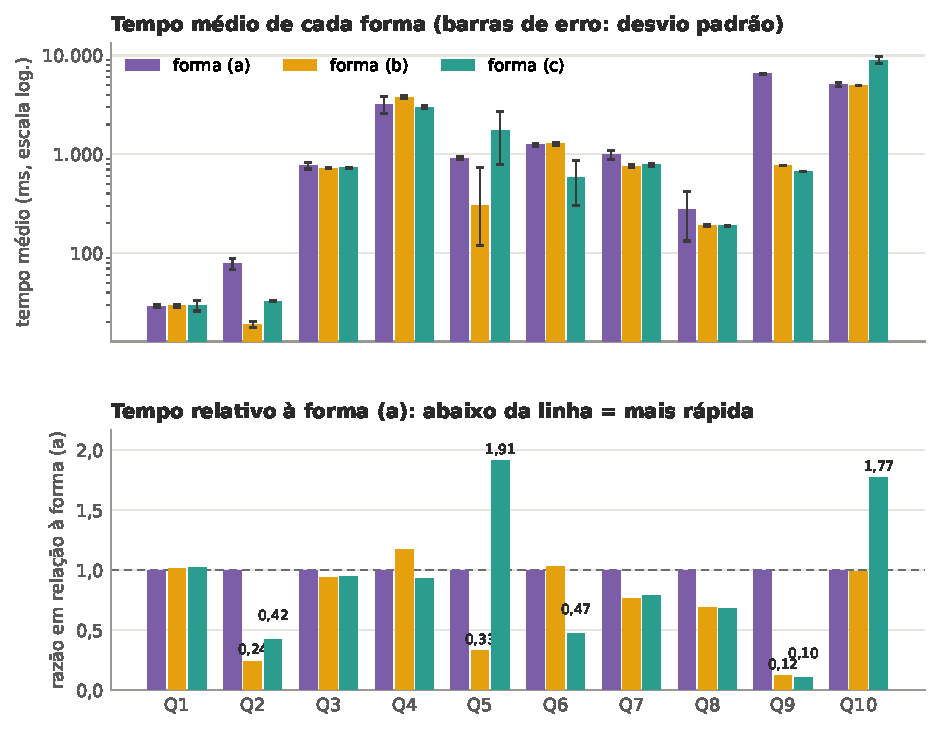
\includegraphics[width=\textwidth]{graficos/comparativo_geral.pdf}
    \caption{Tempo médio de cada forma (em cima, escala log.) e tempo relativo à forma (a) (embaixo; abaixo da linha = mais rápida).}
    \label{fig:tempos}
  \end{minipage}\hfill
  \begin{minipage}[t]{0.42\textwidth}\vspace{0pt}
    \centering
    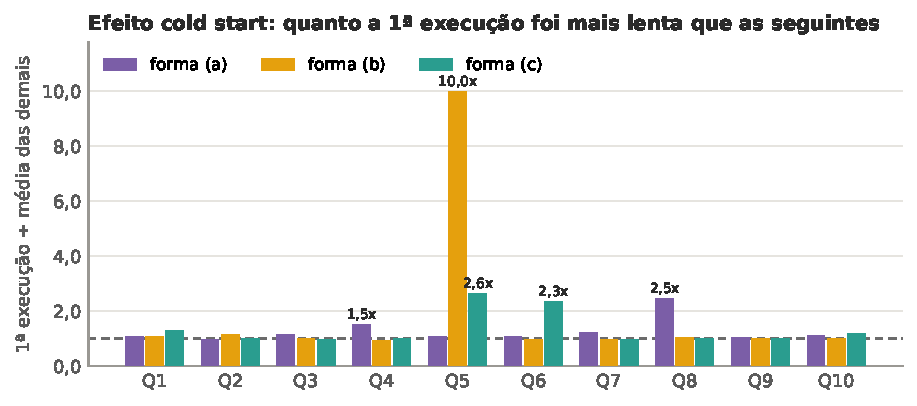
\includegraphics[width=\textwidth]{graficos/cold_start.pdf}
    \caption{Razão entre a 1ª execução e a média das quatro seguintes; acima de 1 indica \emph{cold start}.}
    \label{fig:coldstart}
  \end{minipage}
\end{figure}



\begin{itemize}
  \item \textbf{Índices} trouxeram os maiores ganhos quando o filtro é seletivo numa tabela grande: 4 vezes na Q2, 7 vezes na Q5 e 2,5 vezes na Q6. Não fizeram diferença numa tabela pequena (Q1) e nem sempre foram usados (Q8b). Numa coluna com poucos valores distintos, chegaram a piorar o desempenho (Q10c).
  \item \textbf{Funções aplicadas à coluna} no \texttt{WHERE} impedem a busca por intervalo no índice (Q2c).
  \item \textbf{A ordem das relações no \texttt{FROM}} não importa por si só: o otimizador do MySQL reordena as junções (Q3 e Q8 têm planos idênticos). Forçar uma ordem com \texttt{STRAIGHT\_JOIN} só piorou quando a ordem forçada era pior que a escolhida pelo otimizador (Q4b, Q5c).
  \item \textbf{Formas sintaticamente diferentes podem gerar o mesmo plano.} O MySQL~8 converte \texttt{IN} e \texttt{EXISTS} em semijunções (Q7, Q10b) e incorpora tabelas derivadas à consulta (Q4c). Já \textbf{agregar antes de juntar} foi a reescrita mais eficaz, com ganho de 8 a 10 vezes (Q9).
  \item \textbf{\emph{Cold start}:} a 1ª execução chegou a ser até 9 vezes mais lenta que as seguintes (Q5b), principalmente logo após a criação de um índice. Isso confirma a importância de repetir as medições, e mostra que a mediana é a medida mais estável quando há uma execução discrepante (Figura~\ref{fig:coldstart}).
  \item Em consultas que retornam muitas linhas (Q3, Q4), a \textbf{transferência do resultado} domina o tempo total, o que reduz as diferenças entre as formas.
\end{itemize}



% =====================================================================
\section{Autoavaliação do grupo}\label{sec:autoavaliacao}
% ~0,3 página

\begin{table}[H]
\centering\small
\caption{Tarefas realizadas por integrante.}\label{tab:autoavaliacao}
\begin{tabularx}{\textwidth}{lX}
\toprule
Integrante & Tarefas realizadas \\
\midrule
Gustavo Abalem Tronconi Macedo & \textit{(preencher)} \\
Isabelle de Matos Gonçalves & \textit{(preencher)} \\
Nicolle Salgado Silva & \textit{(preencher)} \\
Paola Alves Ferreira & \textit{(preencher)} \\
\bottomrule
\end{tabularx}
\end{table}

O grupo se organizou em duplas, e as tarefas de cada integrante estão na Tabela~\ref{tab:autoavaliacao}. % completar com um comentário curto sobre a organização

\begin{thebibliography}{9}\small
\bibitem{elmasri} ELMASRI, R.; NAVATHE, S. B. \textit{Sistemas de Banco de Dados}. 6. ed. São Paulo: Pearson Education, 2010.
\bibitem{mysql-explain} ORACLE. \textit{MySQL 8.0 Reference Manual}: EXPLAIN Output Format. Disponível em: \url{https://dev.mysql.com/doc/refman/8.0/en/explain-output.html}.
\bibitem{mysql-indexes} ORACLE. \textit{MySQL 8.0 Reference Manual}: How MySQL Uses Indexes. Disponível em: \url{https://dev.mysql.com/doc/refman/8.0/en/mysql-indexes.html}.
\bibitem{mysql-semijoin} ORACLE. \textit{MySQL 8.0 Reference Manual}: Optimizing IN and EXISTS Subquery Predicates with Semijoin Transformations. Disponível em: \url{https://dev.mysql.com/doc/refman/8.0/en/semijoins.html}.
\bibitem{mysql-derived} ORACLE. \textit{MySQL 8.0 Reference Manual}: Optimizing Derived Tables. Disponível em: \url{https://dev.mysql.com/doc/refman/8.0/en/derived-table-optimization.html}.
\bibitem{mysql-fk} ORACLE. \textit{MySQL 8.0 Reference Manual}: FOREIGN KEY Constraints. Disponível em: \url{https://dev.mysql.com/doc/refman/8.0/en/create-table-foreign-keys.html}.
\bibitem{mysql-check} ORACLE. \textit{MySQL 8.0 Reference Manual}: CHECK Constraints. Disponível em: \url{https://dev.mysql.com/doc/refman/8.0/en/create-table-check-constraints.html}.
\bibitem{mysql-trigger} ORACLE. \textit{MySQL 8.0 Reference Manual}: CREATE TRIGGER Statement. Disponível em: \url{https://dev.mysql.com/doc/refman/8.0/en/create-trigger.html}.
\bibitem{lgpd} BRASIL. Lei nº 13.709, de 14 de agosto de 2018. Lei Geral de Proteção de Dados Pessoais (LGPD).
\bibitem{enunciado} DEPARTAMENTO DE CIÊNCIA DA COMPUTAÇÃO -- UFMG. \textit{Introdução a Banco de Dados: Trabalho Prático 2}. Enunciado. Belo Horizonte, 2026.
\bibitem{material} DEPARTAMENTO DE CIÊNCIA DA COMPUTAÇÃO -- UFMG. \textit{Introdução a Banco de Dados}: material de aula (slides). Disponível no Moodle da disciplina. Belo Horizonte, 2026.
\end{thebibliography}

\end{document}